\chapter{The hydrogen atom}\label{c6}
\section{The Hamiltonian}\label{c6s1}
The quantum mechanical treatment of the hydrogen atom resolved the mystery of 
Bohr's second postulate. It also demonstrated the convenience of the 
Schr\"{o}dinger's approach. His equation can be solved exactly for the hydrogen
atom. The hydrogen atom consists of a single electron in the electric field od a
single proton. Since the electron is almost $1836$ times lighter than the proton
we can, as a first approximation, assume that the proton is at rest. Therefore, 
the energy of the system is
\begin{equation}\label{c6s1e1}
H = \frac{p^2}{2m} - \frac{1}{4\pi\epsilon_0}\frac{e^2}{r},
\end{equation}
where $e$ is the electronic charge and $r$ is the distance between the two. The
operator representation of this Hamiltonian is
\begin{equation}\label{c6s1e2}
\hat{H} = -\frac{\hslash^2}{2m}\nabla^2 - \frac{1}{4\pi\epsilon_0}\frac{e^2}{r}
\end{equation}
and the Schr\"{o}dinger's time independent equation is
\begin{equation}\label{c6s1e3}
-\frac{\hslash^2}{2m}\nabla^2\psi(\vec{r}) - 
\frac{1}{4\pi\epsilon_0}\frac{e^2}{r}\psi(\vec{r}) = E\psi(\vec{r}).
\end{equation}
The spherical symmetry of the problem suggests that we should work in the 
spherical polar coordinate system. The Laplacian in these coordinates is
\begin{equation}\label{c6s1e4}
\nabla^2 = \frac{1}{r^2}\frac{\partial}{\partial r}
\left(r^2\frac{\partial}{\partial r}\right) + 
\frac{1}{r^2\sin\theta}\frac{\partial}{\partial\theta}
\left(\sin\theta\frac{\partial}{\partial\theta}\right) + 
\frac{1}{r^2\sin^2\theta}\frac{\partial^2}{\partial\phi^2}
\end{equation}
The equation \eqref{c6s1e3} is solved using the method of `separation of 
variables'. We write
\begin{equation}\label{c6s1e5}
\psi(\vec{r}) = \psi(r, \theta, \phi) = R(r)\Theta(\theta)\Phi(\phi)
\end{equation}
so that equation \eqref{c6s1e3} becomes
\begin{eqnarray}
-\frac{\hslash^2}{2m}\left[
\frac{\Theta\Phi}{r^2}\frac{d}{dr}\left(r^2\frac{dR}{dr}\right) +
\frac{R\Phi}{r^2\sin\theta}\frac{d}{d\theta}
\left(\sin\theta\frac{d\Theta}{d\theta}\right) + 
\frac{R\Theta}{r^2\sin^2\theta}\frac{d^2\Phi}{d\phi^2}\right] &=& \nonumber \\ 
\left(E + \frac{1}{4\pi\epsilon_0}\frac{e^2}{r}\right)R\Theta\Phi & & 
\label{c6s1e6}
\end{eqnarray}
Multiplying both sides by
\[
\frac{r^2\sin^2\theta}{R\Theta\Phi}
\]
and rearranging a bit, we get
\begin{equation}\label{c6s1e7}
\frac{\sin^2\theta}{R}\frac{d}{dr}\left(r^2\frac{dR}{dr}\right) +
\frac{\sin\theta}{\Theta}\frac{d}{d\theta}
\left(\sin\theta\frac{d\Theta}{d\theta}\right) +
\frac{2m}{\hslash^2}\left(E + \frac{e^2}{4\pi\epsilon_0 r}\right)
r^2\sin^2\theta =
-\frac{1}{\Phi}\frac{d^2\Phi}{d\phi^2}. 
\end{equation}
The left hand side of this equation is a function of $r$ and $\theta$ while
the right hand side depends on $\phi$ alone. Therefore, each side must be equal
to a constant, say $\alpha$. In particular, we get
\begin{equation}\label{c6s1e8}
\frac{1}{\Phi}\frac{d^2\Phi}{d\phi^2} = -\alpha
\end{equation}
or
\begin{equation}\label{c6s1e9}
\frac{d^2\Phi}{d\phi^2} + \alpha\Phi = 0.
\end{equation}
This equation will have a periodic solution if $\alpha > 0$ and an exponential
one if $\alpha < 0$. The hydrogen atom is clearly periodic in $\phi$. Therefore,
we can write
\begin{equation}\label{c6s1e10}
\alpha = m_l^2
\end{equation} 
so that we get
\begin{equation}\label{c6s1e11}
\frac{d^2\Phi}{d\phi^2} + m_l^2\Phi = 0
\end{equation}
and
\begin{equation}\label{c6s1e12}
\frac{\sin^2\theta}{R}\frac{d}{dr}\left(r^2\frac{dR}{dr}\right) +
\frac{\sin\theta}{\Theta}\frac{d}{d\theta}
\left(\sin\theta\frac{d\Theta}{d\theta}\right) +
\frac{2m}{\hslash^2}\left(E + \frac{e^2}{4\pi\epsilon_0r}\right)
r^2\sin^2\theta = m_l^2.
\end{equation}
The solution of the equation \eqref{c6s1e11} is
\begin{equation}\label{c6s1e13}
\Phi(\phi) = \alpha_1 e^{im_l\phi} + \alpha_2 e^{-im_l\phi},
\end{equation}
where $\alpha_1$ and $\alpha_2$ are constants of integration. Since $\Phi(\phi)
= \Phi(\phi + 2\pi)$ $m_l$ must be an integer. We can therefore write the 
solution \eqref{c6s1e13} as just
\begin{equation}\label{c6s1e14}
\Phi_{m_l}(\phi) = \alpha_1 e^{im_l\phi}
\end{equation}
as the other factor is automatically included in the first one. $m_l$ is called
the \emph{magnetic quantum number} and it is an integer. In order to separate 
equation \eqref{c6s1e12}, divide both sides by $\sin^2\theta$ and rearrange a 
bit to get
\begin{equation}\label{c6s1e15}
\frac{1}{R}\frac{d}{dr}\left(r^2\frac{dR}{dr}\right) +
\frac{2m}{\hslash^2}\left(E + \frac{1}{4\pi\epsilon_0}\frac{e^2}{r}\right)r^2 =
-\frac{1}{\Theta\sin\theta}\left(\sin\theta\frac{d\Theta}{d\theta}\right) +
\frac{m_l^2}{\sin^2\theta}.
\end{equation}
Once again we have a situation in which the left hand side of the equation 
depends on one variable, $r$, and the right hand side on another, $\theta$
so that each side is a constant, say $\beta$. Thus, we have
\begin{equation}\label{c6s1e16}
-\frac{1}{\Theta\sin\theta}\frac{d}{d\theta}
\left(\sin\theta\frac{d\Theta}{d\theta}\right) +\frac{m_l^2}{\sin^2\theta} = 
\beta
\end{equation}
and
\begin{equation}\label{c6s1e17}
\frac{1}{R}\frac{d}{dr}\left(r^2\frac{dR}{dr}\right) +
\frac{2m}{\hslash^2}\left(E + \frac{1}{4\pi\epsilon_0}\frac{e^2}{r}\right)r^2 =
\beta.
\end{equation}
We will solve these equations in the following sections. And yet, before 
proceeding we notice that the energy $E$ is part of the $r$-equation. This 
indicates that the energy of an electron in the Hydrogen atom depends on $r$
alone, in agreement with the Bohr model.

\section{The $\theta$ and $r$ equations}\label{c6s2}
Equations \eqref{c6s1e6} and \eqref{c6s1e7} can be solved using the Frobenius
series solution method however the analysis is a bit labourious. We will,
therefore, only summarise it here. The solutions of \eqref{c6s1e16} remain 
finite as $\theta \rightarrow 0$ and $\theta \rightarrow \pi$ only if $\beta$
is of the form $l(l+1)$ for a positive integer $l$. When $m_l = 0$, the 
solutions of \eqref{c6s1e16} are called Legendre polynomials. When $m_l \le 0$,
they are required to be such that $-l \le m_l \le l$ and the corresponding
solutions are called associated Legendre polynomials. The product of the 
solution of the $\theta$ equation and \eqref{c6s1e14} is called a spherical
harmonic of order $l$ and $m_l$. Spherical harmonics were studied as solutions
of Laplace equation since a century prior to the advent of quantum mechanics.
The Legendre polynomials for are denoted by $P_l(\cos\theta)$ and the associated
Legendre polynomials by $P_l^{m_l}(\cos\theta)$. The spherical harmonics are
denoted by
\begin{equation}\label{c6s1e18}
Y_{l, m_l}(\theta, \phi) = N_{lm_l}P_l^{m_l}(\cos\theta)\Phi_{m_l}(\phi).
\end{equation}
$l$ is called the \emph{orbital quantum number} and it restricts the values 
$m_l$ can take. Likewise, the solution of the $r$ equation can be written in 
terms of the associated Laguerre polynomials. The solutions exist for all 
$E \ge 0$ but for $E < 0$, they exists only for the discrete set
\begin{equation}\label{c6s1e19}
E_n = -\frac{me^4}{32\pi^2 n^2\hslash^2\epsilon_0^2} = 
-\frac{me^4}{8n^2h^2\epsilon_0^2},
\end{equation}
where $n \ge 0$ is an integer and it is always greater than $l$. It is called
the \emph{principal quantum number}.

Thus the three equations, one each for $r$, $\theta$ and $\phi$ give rise to the
quantum numbers $n, l, m_l$ such that
\begin{eqnarray}
n &\ge& 0 \label{c6s2e3} \\
l &<& n \label{c6s2e4} \\
|m_l| &\le& l \label{c6s2e5}
\end{eqnarray}
Equation \eqref{c6s2e5} can be written in an equivalent form
\begin{equation}\label{c6s2e6}
-l \le m_l \le l.
\end{equation}

\subsection{Problem set 1}
\begin{enumerate}
\item Consider a thought experiment in which the electrostatic potential was of
the form $e^{-r}$. Which of the three quantum numbers introduced above would 
have remained unchanged.
\item Show that there are $n^2$ electrons with principal quantum number $n$.
You may remember having learnt that this number is $2n^2$. The factor of $2$
is missing in our analysis because we still have not take into account the spin
of an electron.
\item Although the proton is $1836$ times heavier than an electron, it does get
affected by the reaction of the electron. What would change in our analysis if
we want to take the proton's motion into account? (Hint: problem 4 in chapter
\ref{c3}.)
\end{enumerate}

\section{Quantization of angular momentum}\label{c6s3}
Bohr's second postulate was about the quantization of the electron's angular 
momentum. We will now show that it is possible to understand it in the framework
of quantum mechanics. The angular momentum is an important dynamical variable
in quantum mechanics with a rich theory which explains its quantization in a
very natural way. We will not discuss it in this course and instead restrict
our analysis to hydrogen atom alone.

Since $\beta = l(l+1)$, we can rearrange equations \eqref{c6s1e6} and 
\eqref{c6s1e7} as 
\begin{eqnarray}
\frac{1}{\sin\theta}\frac{d}{d\theta}
\left(\sin\theta\frac{d\Theta}{d\theta}\right) + 
\left(\frac{m_l^2}{\sin^2\theta} - l(l+1)\right)\Theta &=& 0 \label{c6s3e1} \\
\frac{1}{r^2}\frac{d}{dr}\left(r\frac{dR}{dr}\right) + \frac{2m}{\hslash^2}
\left[\left(E + \frac{1}{4\pi\epsilon_0}\frac{e^2}{r}\right)
- \frac{l(l+1)\hslash^2}{2mr^2}\right]R &=& 0 \label{c6s3e2}
\end{eqnarray}
The $r$-equation should ideally not have anything to do with the orbital motion.
Therefore, the presence of the term $l(l+1)\hslash^2/(2mr^2)$ is a bit 
disconcerting. The total energy $E$ is the sum of the electron's potential
energy and kinetic energy. The former is $-e^2/(4\pi\epsilon_0 r)$, while the 
latter can be written as the sum of $T_r$, the radial, and $T_o$, the orbital
kinetic energies. We conjecture that the orbital kinetic energy is
\begin{equation}\label{c6s3e3}
T_o = \frac{l(l+1)\hslash^2}{2mr^2}
\end{equation}
so that there is no dependence of the orbital motion on the $r$-equation. If
$v_o$ is the orbital velocity then 
\begin{equation}\label{c6s3e4}
T_o = \frac{mv_o^2}{2}
\end{equation}
so that from \eqref{c6s3e3} and \eqref{c6s3e4} we get
\begin{equation}\label{c6s3e5}
mv_or = \sqrt{l(l+1)}\hslash.
\end{equation}
Although the angular momentum is not an integral multiple of $\hslash$ as Bohr
had proposed, it is quantized nevertheless.

\section{Electron density}\label{c6s4}
The squared modulus solution of \eqref{c6s1e6} is the probability density 
function of finding an electron in the atom. Although the mathematical forms 
of the wave-function and its modulus are quite formidable their plots are quite
familiar to us. The figure \ref{c6f1} labels the probability densities by the
triple $(n, l, m_l)$ of the quantum numbers. Wave functions with different 
values of $l$ are called orbitals. The orbitals with $l = 0$ have a spherical 
symmetry.  They are called s-orbitals. Observe the one with $n=2$. The orbital 
has minumum, between two maxima of unequal sizes. The surfaces in which the 
orbitals are zero are called nodal surfaces. Thus, the $2s$ orbital has a nodal 
surface between the two maxima. The orbitals with $l = 1$ are called the p-
orbitals. They have two lobes separated by a nodal plane. The orbitals with 
$l = 2$ are called d-orbitals and those with $l = 3$ are called f-orbitals. 
They have far more complicated shapes. Their shapes play an important role in 
inorganic chemistry, especially of the transition elements.

The diagram in figure \ref{c6f1} also gives an expression for the wavefunction.
The variable $\rho$ in it is the ratio $r/a_0$, where $a_0$ is the radius of the
first Bohr orbit. The factor $e^{-\rho}$ ensures that the wavefunction goes to
zero away from the nucleus. The angular distribution of the orbitals is 
determined solely by the spherical harmonics and the radial distribution by the
associated Laguerre polynomials (and $e^{-\rho}$).
\begin{figure}
\begin{center}
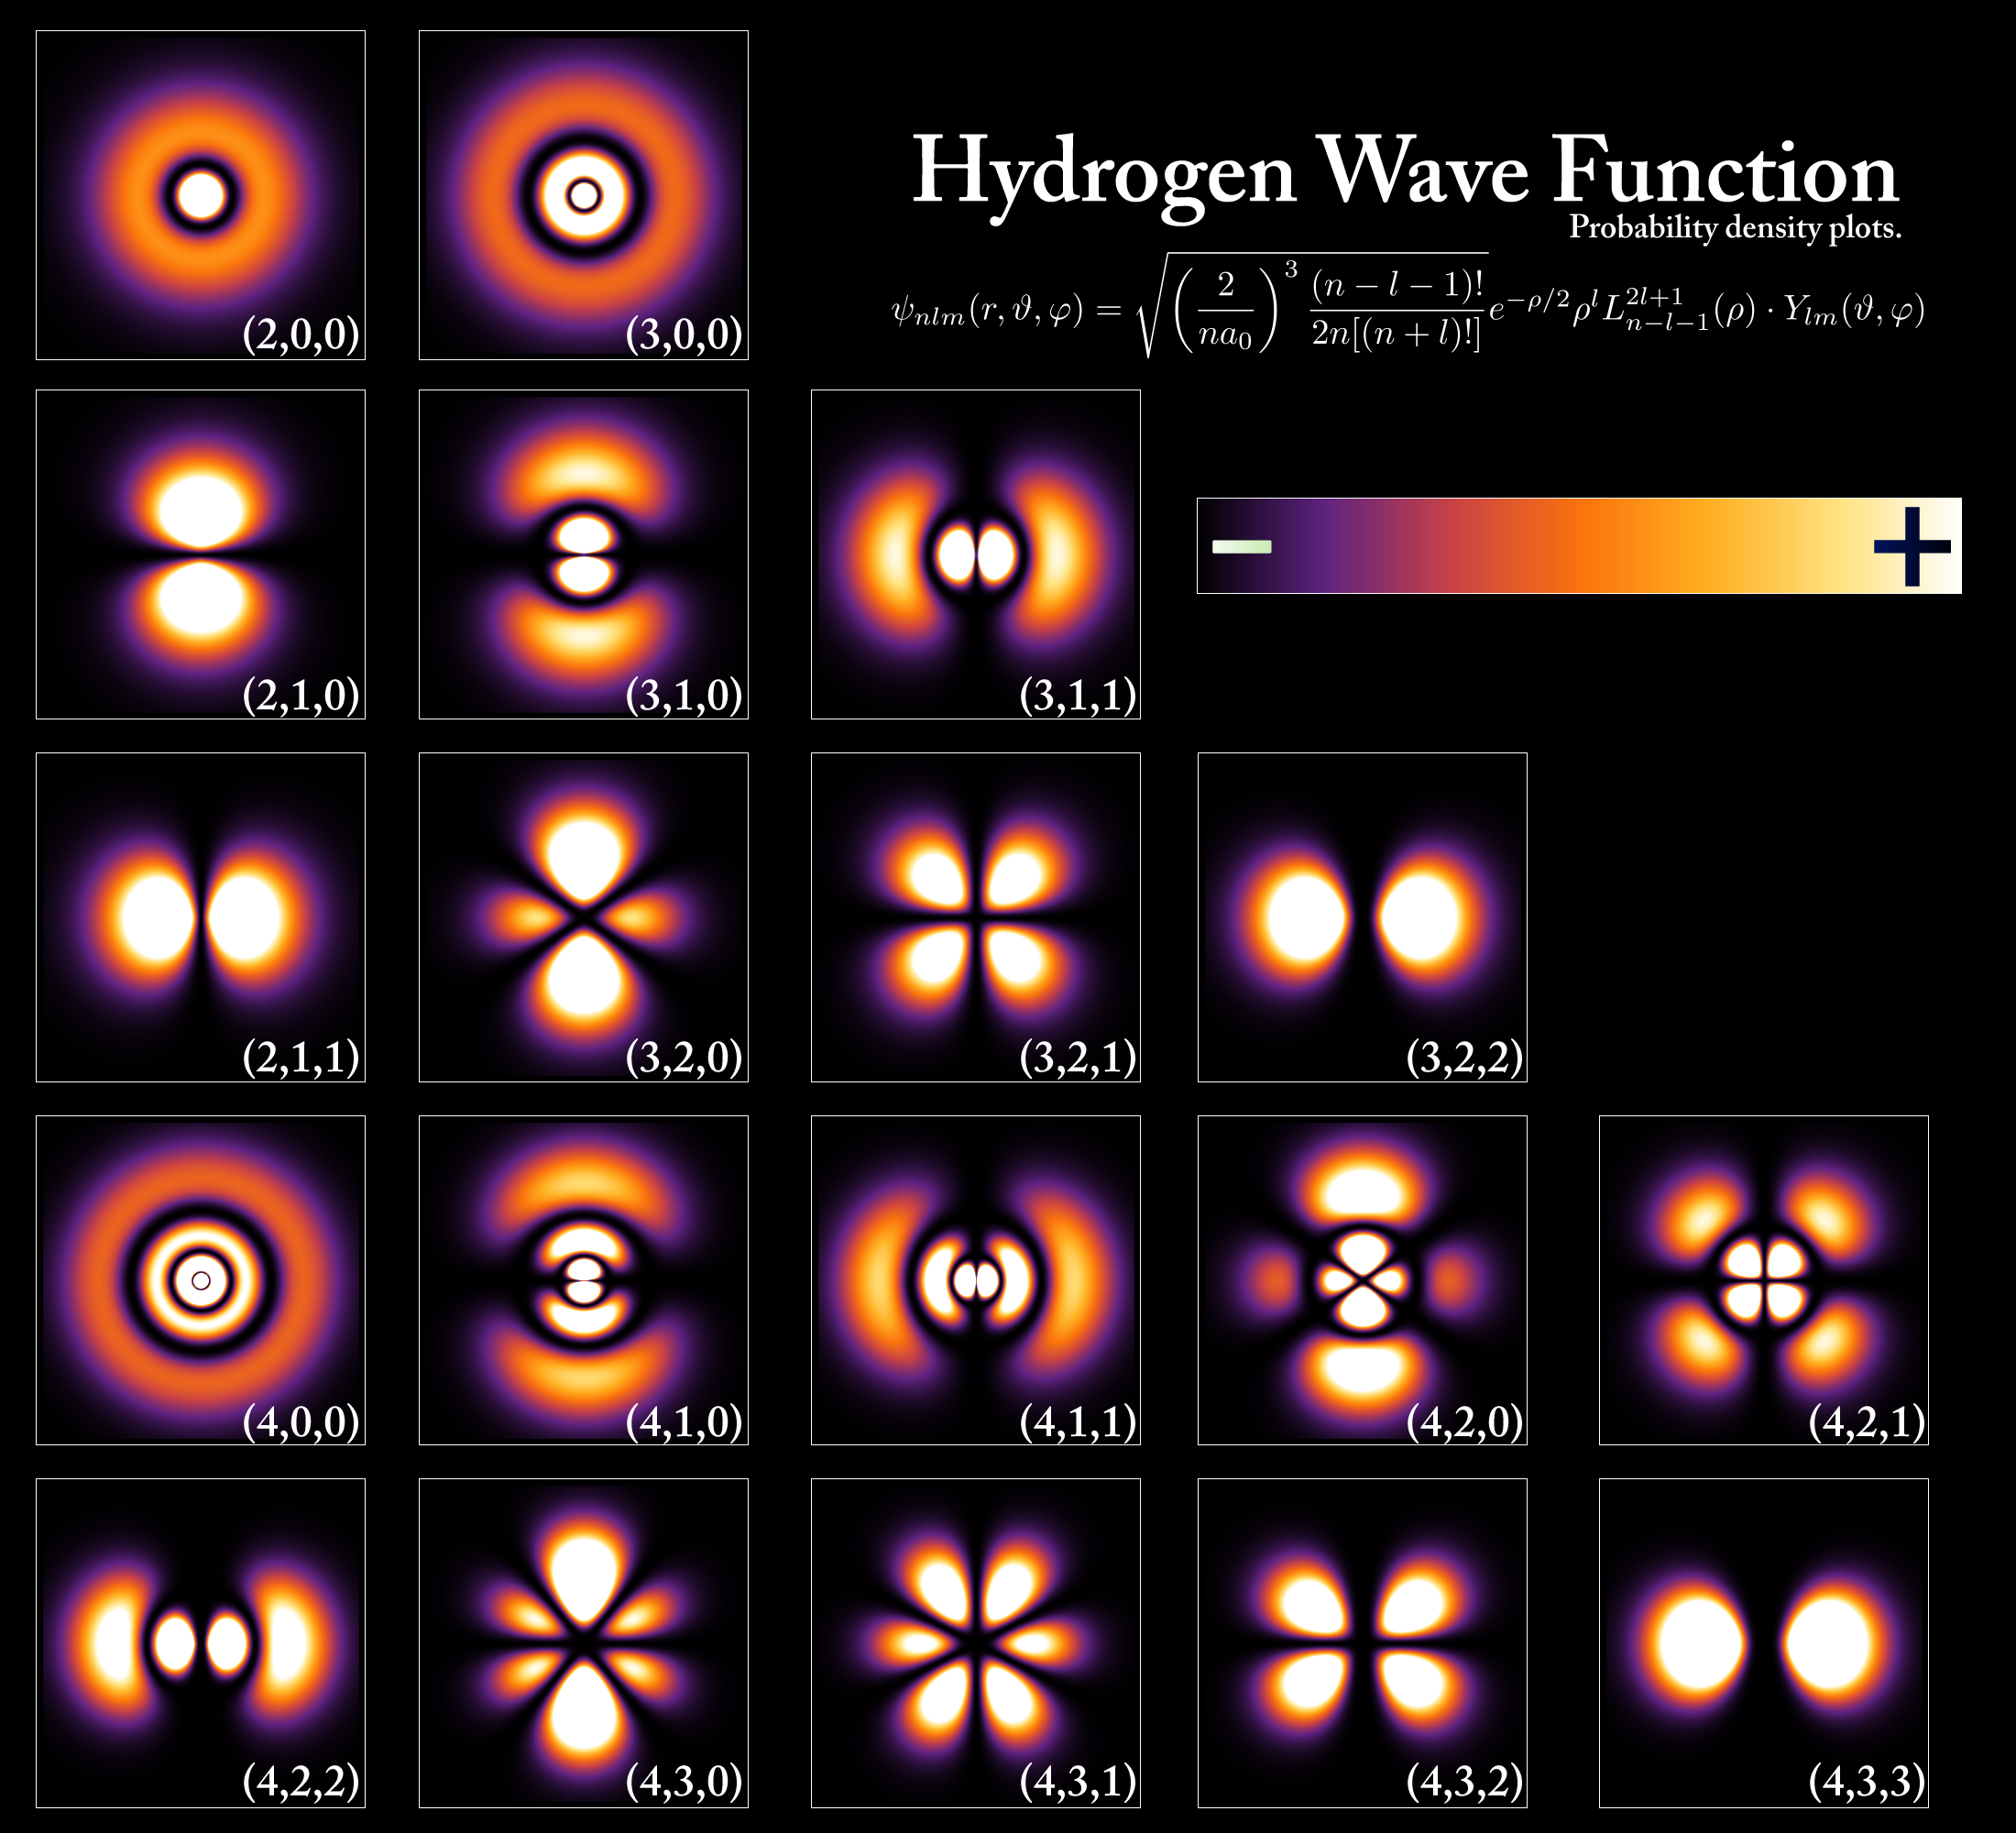
\includegraphics[scale=0.20]{Hydrogen_Density_Plots}
\caption{Hydrogen orbitals credit: Wikipedia}
\label{c6f1}
\end{center}
\end{figure}

\subsection{Problem set 2}
\begin{enumerate}
\item Based on your understanding of the solutions of the $r, \theta$ and 
$\phi$ equations show that the $|\psi|^2$ is independent of the azimuthal angle
$\phi$. How do you decide where the $z$-axis is?
\item The wavefunction for the $n=1, l=0, m_l=0$ is
\begin{equation}\label{c6s3e6}
\psi_{1,0,0}(r,\theta,\phi) = \frac{e^{-r/a_0}}{\sqrt{\pi}a_0^{3/2}}.
\end{equation}
Let $P(r)$ be the probability density of finding an electron in the thin 
spherical shell with radii $r$ and $r + dr$. Then,
\begin{equation}\label{c6s3e7}
P(r) = \int_0^{\pi}\int_0^{2\pi}|\psi_{1,0,0}^2|^2r^2\sin\theta d\theta d\phi.
\end{equation}
Show that
\begin{equation}\label{c6s3e8}
P(r) = \frac{4r^2 e^{-r/a_0}}{a_0^3}.
\end{equation}
Hence show that $P$ has a maximum at $r = a_0$, where $a_0$ is the radius of the
first Bohr orbit.
\end{enumerate}
